\documentclass[12pt,a4paper]{article}
\usepackage[utf8]{inputenc}
\usepackage[spanish]{babel}
\usepackage{graphicx}
\usepackage{kpfonts}
\usepackage[left=2cm,right=2cm,top=2cm,bottom=2cm]{geometry}
\begin{document}
\title{Universidad politecnica\\ de la \\ Zona Metropolitana\\ de Guadalajara}
\author{Tarea 3\\ Angel Eraclio Briano Garcia 18311625\\ Ing. Mecatronica 4B}
\maketitle
\begin{figure}[h!]
\centering

\includegraphics[scale=1]{untitled.png} 
\end{figure}
\newpage
\title{\textbf{Arreglos y parametros de los amplificadores de clase A:}\\ \\ }
Amplificador clase A. Son aquellos amplificador cuyas etapas de potencia consumen corrientes altas y continuas de su fuente de alimentación, independientemente de si existe señal de audio o no.\\
\begin{figure}[h!]
\centering
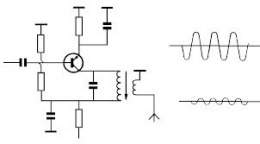
\includegraphics[scale=1]{260px-AmplificadorclaseA.jpg} 
\end{figure}\\
Un amplificador de potencia funciona en clase A cuando la tensión de polarización y la amplitud máxima de la señal de entrada poseen valores tales que hacen que la corriente de salida circule durante todo el período de la señal de entrada.\\
La corriente de salida circula durante todo el ciclo de la señal de entrada, en un solo transistor. La corriente de polarización del transistor de salida es alta y constante durante todo el proceso, independientemente de si hay o no hay salida de audio. La distorsión introducida es baja a niveles muy bajos de señales (para niveles altos las distorsiones de segundo orden son importantes) , el rendimiento también será bajo, estando siempre por debajo del 50 porciento, lo que significa que la otra mitad de la corriente amplificada será disipada por el transistor en forma de calor. Los amplificadores de clase A se utilizan solo en etapas preamplificadoras , su bajo rendimiento y su elevado nivel de distorsión armónica no lo hacen aptos para etapas de potencia. La curva de transferencia de un transistor NO ES LINEAL , en un amplificador de este tipo la parte lineal de dicha curva es la limitante al tener que trabajar con señales altas , en un amplificador clase B o AB en configuración push pull la señal eléctrica se amplifica en semiciclos separados aumentando así la capacidad lineal de transferencia (menor distorsiones , distorsiones de segundo orden casi nulas) y mayor eficiencia.
\newpage


\section{Caracteristicas de los amplificadores de clase A \\ }
Esta amplificación presenta el inconveniente de generar una fuerte y constante emisión de calor. No obstante, los transistores de salida están siempre a una temperatura fija y sin alteraciones.
Se afirma que esta clase de amplificación es frecuente en circuitos de audio y en los equipos domésticos de gama alta, ya que proporcionan una calidad de sonido potente y de muy buena calidad.\\
\begin{figure}[h!]
\centering
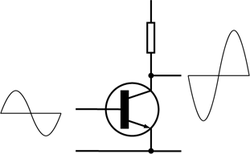
\includegraphics[scale=1]{250px-Electronic_Amplifier_Class_A.png} 
\end{figure}\\
Los amplificador de clase A a menudo consisten en un transistor de salida conectado al positivo de la fuente de alimentación y un transistor de corriente constante conectado de la salida al negativo de la fuente de alimentación.
La señal del transistor de salida modula tanto el voltaje como la corriente de salida. Cuando no hay señal de entrada, la corriente de polarización constante fluye directamente del positivo de la fuente de alimentación al negativo, resultando que no hay corriente de salida, se gasta mucha corriente.\\ 
\newpage
En los amplificadores de clase A no hay nunca corriente de reja (base) por lo que es indiferente decir que el amplificador es de clase A1 o de clase A. Lo contrario ocurre en los amplificadores de clase C donde siempre va a existir corriente de reja (base), en este caso es indiferente decir que el amplificador es de clase C2 o de clase C (a secas).\\
\section{Ventajas}
La clase A se refiere a una etapa de salida con una corriente de polarización mayor que la máxima corriente de salida que dan, de tal forma que los transistores de salida siempre están consumiendo corriente. La gran ventaja de la clase A es que es casi lineal, y en consecuencia la distorsión es menor.

\section{Desventajas}
La gran desventaja de la clase A es que es poco eficiente, se requiere un amplificador de clase A muy grande para dar 50 W, y ese amplificador usa mucha corriente y se pone a muy alta temperatura.
\begin{figure}[h!]
\centering
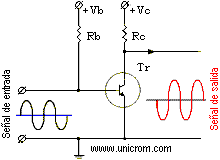
\includegraphics[scale=1]{images.png} 
\end{figure}\\


\end{document}